\section{Задание 5}

\begin{enumerate}
	\item Пусть $X_i \sim \mathcal{N}(\mu, \sigma^2)$. Убедиться эмпирически в 
	справедливости ЗБЧ и ЦПТ, т.е. исследовать поведение суммы $S_n$ и 
	эмпирического распределения величины
	\begin{equation*}
		\frac{S_n - \mu n}{\sigma \sqrt{n}}.
	\end{equation*}
	\item Считая $\mu$ и $\sigma^2$ неизвестными, для пункта 1 построить 
	доверительные интервалы для среднего и дисперсии.
	\item Пусть $X_i \sim K(a, b)$ имеет распределение Коши со сдвигом $a$ и 
	масштабом $b$. Проверить эмпирически, как ведут себя суммы $S_n/n$. 
	Результат объяснить, а также найти закон распределения данных сумм.
\end{enumerate}

\subsection{Проверка ЗБЧ и ЦПТ}
	Действительно, для выборки $\{X_i\} \sim \mathcal{N}(\mu,\sigma^2)$ значение 
	$\dfrac{S_n}{n} = \dfrac{\sum_{i=1}^n X_i}{n}$ ведет себя в соответствии с 
	законом больших чисел (см. рис. \ref{LLN}), т.е
	\begin{equation*}
		\frac{S_n}{n} \rightarrow \mu \text{, при } n \rightarrow \infty.
	\end{equation*}

	Результаты опыта соответствуют и центральной пределной теореме, т.е
	\begin{equation*}
		\frac{S_n - \mu n}{\sigma \sqrt{n}} \xrightarrow{d} \eta \sim 
		\mathcal{N}(0,1) \text{ при } n \rightarrow \infty. 
		\text{ (см. рис. \ref{CLT})}
	\end{equation*}

	\begin{figure}[tbp]
        \centering
        \begin{subfigure}[b]{0.45\textwidth}
            \centering
            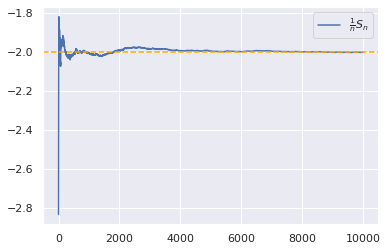
\includegraphics[width=\textwidth]{resources/task5_LLN.png}
            \caption{ЗБЧ ($\mu = -2,\:\sigma^2 = 0.5$)}
            \label{LLN}
        \end{subfigure}
        \hfill
        \begin{subfigure}[b]{0.5\textwidth}
            \centering
            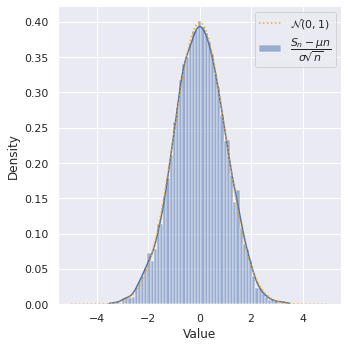
\includegraphics[width=\textwidth]{resources/task5_CLT.png}
            \caption{ЦПТ ($\mu = -2,\:\sigma^2 = 0.5$)}
            \label{CLT}
        \end{subfigure}
        \caption{}
    \end{figure}
	
\subsection{Доверительные интервалы}
	Пусть имеется выборка $X_i \sim \mathcal{N}(\mu, \sigma^2)$, где $\mu$ и 
	$\sigma^2$~--- неизвестны. Исходя из
	\begin{theorem} Для нормальной выборки $X_i \sim \mathcal{N}(\mu, \sigma^2)$
	выборочное среднее $\overline X = \frac{1}{n}\sum X_i$ и выборочная 
	дисперсия $S^2 = \frac{1}{n}\sum (X_i-\overline X)^2$ независимы, причем 
	$nS^2/\sigma^2 \sim \chi_{n-1}^2$, а $\sqrt{n-1}(\overline X - \mu)/S 
	\sim t_{n-1}$.
	\end{theorem}
	можно построить доверительные интервалы 
	\begin{itemize}
		\item для параметра сдвига $\mu$:
		\[\Prb{\overline X - \frac{y_{1-\alpha/2}S}{\sqrt{n-1}} < \mu < 
		\overline X - \frac{y_{\alpha/2}S}{\sqrt{n-1}}} = 
		\Prb{y_{\alpha/2} < \frac{\sqrt{n-1}(\overline X - \mu)}{S} < 
		y_{1-\alpha/2}} = 1-\alpha,\]
		где $y_p$~--- $p$-квантиль распределения Стьюдента $t_{n-1}$ (в силу 
		симметрия закона $y_{\alpha/2} = -y_{1-\alpha/2}$);
		\item и для параметра масштаба $\sigma$:
		\[\Prb{\frac{\sqrt{n}S}{\sqrt{z_{1-\alpha/2}}} < \sigma < 
		\frac{\sqrt{n}S}{\sqrt{z_{\alpha/2}}}} = \Prb{z_{\alpha/2} < 
		\frac{nS^2}{\sigma^2} < z_{1-\alpha/2}} = 1-\alpha,\]
		где $z_p$~--- $p$-квантиль закона $\chi_{n-1}^2$.
	\end{itemize}

	Доверительные интервалы для некотрой выборки из $\mathcal{N}(-2,0.5)$ для 
	разных $n$ приведены на рис. \ref{CI}	

	\begin{figure}[tbp]
        \centering
        \begin{subfigure}[b]{0.47\textwidth}
            \centering
            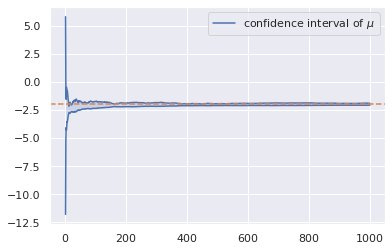
\includegraphics[width=\textwidth]{resources/task5_CI_mu.png}
            \caption{}
            \label{CI_mu}
        \end{subfigure}
        \hfill
        \begin{subfigure}[b]{0.45\textwidth}
            \centering
            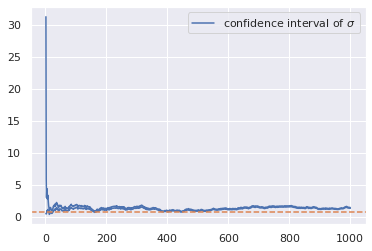
\includegraphics[width=\textwidth]{resources/task5_CI_sigma.png}
            \caption{}
            \label{CI_sigma}
        \end{subfigure}
        \caption{} \label{CI}
    \end{figure}

\subsection{Поведение сумм $S_n/n$ для распределения Коши}
	Как известно распределение Коши не имеет математического ожидания (ни 
	конечного, ни бесконечного), а потому для него не выполяется ЗБЧ, и 
	сходимость выборочного среднего $S_n/n$ не имеет места. Тем не менее 
	распределение $\mathrm{Cauchy}(a,b)$ симметрично относительно $a$ и интеграл 
	$\int\limits_{-\infty}^{\infty} x p_{c}(x)\, dx$ сходится  в смысле главного 
	значения к $a$. Этими наблюденями объясняется полученное на опыте поведение
	сумм $S_n/n$: их значение в основном держится около некоторой средней 
	величины определяемой значением $a$ (сходимость $v.p.$) и "периодическими" 
	сильными выборосами (расходимость в целом) от $a$ ее отклонившими. График 
	сумм $S_n/n$ для некоторой выборки $X_i$ представлен на 
	рис. \ref{cauchy_sums}.

	\begin{figure}[tbp]
        \centering
        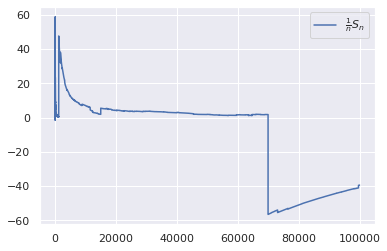
\includegraphics[width=0.5\textwidth]{resources/task5_cauchy.png}
        \caption{$a=0, b=3$}
        \label{cauchy_sums}
    \end{figure}

	Ввиду отстутствия математического ожидания не выполнена и ЦПТ, и сходимость 
	$S_n/n$ по распределению с ее помощью доказать не получится. Вместо этого 
	воспользуемся аппаратом характеристических функций. Характеристическая 
	функция распределения Коши с параметрами $a$, $b$ имеет вид
	\begin{equation*}
		\psi(t) = 
		\int\limits_{-\infty}^{\infty} \frac{e^{itx}}{\pi(b^2 + (x-a)^2)} \,dx =
		e^{ait-b|t|}.
	\end{equation*}
	Характеристическая функция суммы независимых случайных величин есть 
	произведение их характеристических функций, а потому
	\begin{equation} \label{char_fun}
		\psi_{\frac{S_n}{n}}(t) = \psi_{\sum \frac{1}{n} X_i} (t) = 
		\prod \psi_{\frac{1}{n} X_i} (t) = \prod \psi_{X_i} (\tfrac{t}{n}) = 
		e^{n(ai\frac{t}{n}-b|\frac{t}{n}|)} = e^{ait-b|t|}.
	\end{equation}
	Поскольку хар. функция однозначно задает распределение, равенство 
	\eqref{char_fun} доказывет что величина $\frac{S_n}{n}$ (так же как и 
	${X_i}$) распределена по Коши с параметрами $a$ и $b$.